\chapter{Implementation Details}
\label{chapter:eleven}

%The history of Scale Space tracks back to Witkin 1983, where it was applied to time series.  He highlighted the Spatial Coincidential assumption.
%Basically, the number of zero crossing of the first derivative is reduced with increasing scale.
%
%\begin{story}[Biomimetic Applications]
%
%\end{story}
%
%This method is actually composed on two submethods: the first is the keypoint localization, while the second is the histogram of gradient orientations, which is the basis for this thesis.
%
%bla bla bla
%
%
%Aca también voy a mandar detalles de la implementacion.   como por ejemplo los detalles de como funciona vlfeat y las modificaciones.

\section{Open Source Software}
The software produced for this Thesis can be found in the following public repositories:

\begin{enumerate}
\item \url{https://bitbucket.org/itba/hist}\label{HistRepo}
\item \url{https://github.com/faturita/BciVisualToolbox}\label{BciVisualToolbox}
\item \url{https://github.com/faturita/vlfeat}\label{VLFeat}
\item \url{https://github.com/faturita/GuessMe}\label{GuessMe}
\end{enumerate}

\vspace{2pt}

Repository~\ref{HistRepo} contains an integrated version of the whole set of utilities. It is available under GPL license.

\section{BCI and EEG Utilities}

Signal Processing, EEG processing routines and BCI utilities have been made publicly available in the Repository~\ref{BciVisualToolbox}.  This package is a set of tools for MATLAB (Mathworks Inc., Natick, MA, USA).  It is compatible with MATLAB V2014a and has been tested successfully on 2015b and 2017a, on Windows 7 and Mac OS X High Sierra.

%\begin{lstlisting}[language=octave]
%[image, DOTS, zerolevel] = eegimage
%	(channel,EEGsignal,gamma,gammat, 
%	drawzerolevel,defaultheight,pixelcolorinverted,interpolate)
%\end{lstlisting}

\section{VLFeat}

In order to process the image, extract the patch, obtain the gradient image and the SIFT Descriptor, the Histogram of Gradient Orientations the VLFeat~\cite{Vedaldi2010} library is used.   This library was modified to adapt it to process signal plots and the code has been made available at the public Repository~\ref{VLFeat}. 

The implemented changes are subtle modifications of the standard SIFT Descriptor~\cite{Rey-Otero2014}, and modifications on the particular implementation provided by this library.  The following sections describe each one of these changes.

\subsection{SIFT Detector and Custom Patch}

The SIFT Detector is not being used in this implementation.  Hence, the keypoint location and patch parameters are directly provided to the VLFeat library to calculate the SIFT Descriptor.  The \textit{frame} is a data structure composed of keypoint center location  $(x_{kp}, y_{kp})$, patch scale  $S$ and patch orientation $\theta$: $ ( x_{kp}, y_{kp}, S, \theta ) $. These parameters are the output of the SIFT Detector.  The code provided in Repository~\ref{BciVisualToolbox} calculates these frames based on the provided parameters and on the structure of the EEG signal.

\subsection{Patch Scale}

Whereas in the standard SIFT implementation the patch is a squared region and there is only one SIFT scale parameter, in this implementation the scale is divided in two: $\gls{St}$ and $\gls{Sv}$.  This is a very important modification because otherwise signal plots, which may extend only on the horizontal direction, would not have been able to be mapped.  Using a rectangular frame there isn't any constraint on its size and it can be adjusted at will to map any waveform.

This modification forces the frame to be also altered to incorporate one extra parameter, the extra scale.  The frame is thus composed of: $ ( x_{kp}, y_{kp}, \gls{St}, \gls{Sv}, \theta ) $.  

\subsection{Patch Orientation}

The value $\theta$ is the patch orientation which does not provide any extra utility so far for the extraction of characteristics from plots.  The orientation of the patch is fixed to zero (vertical, pointing upwards or towards the horizontal axis of the image coordinate system in Figure~\ref{fig:imagecoordinatesystem}).

\subsection{Patch Size in Pixels}

The nominal size of a patch in many SIFT implementations is $4 \times m \times S$, with $m$ being the magnification factor and $S$ being the SIFT scale.  However due to the trilinear interpolation, pixels that are located outside the nominal patch size are also considered to calculate the histogram, and the patch boundary is loosely defined between implementations.  In this case, the waveform must be accurately delimited, hence the effective size of the patch must to be considered. This size is indeed based on the unit-scale constant and it is $\gls{Deltas} = \sqrt{2} \; m \; 5$.  The magnification factor $m$ is set as $3$ and $5$ is the result of using $4$ blocks on each direction plus half a block on each side.  For a unit scale on vertical and horizontal direction, this gives an effective patch size of $22$ pixels on both directions.

The VLFeat libraries in Repository~\ref{VLFeat} for Matlab that show the patch superimposed on the images are modified to account for this effective patch size.

\subsection{Octave Selection}

A gradient image is used to calculate the oriented gradients and reckon the histogram of gradient orientations.   SIFT calculates different octaves downsampling the original image and applying a Gaussian smoothing operation increasing the sigma parameter of the Gaussian window step by step.  SIFT calls \textit{octave} to each downsampling level~\cite{Lowe2004,Rey-Otero2014}. VLFeat estimates the octave to use on the gradient image based on the image size and patch parameters.   This is modified in this implementation to use only the zero octave which means that the gradient image has the same size as the original patch, without downsampling.

\subsection{First Octave Smoothing}

Additionally, the VLFeat implementation performs a Gaussian blurring on the gradient image regardless of the octave.  This is disabled in this implementation.

\subsection{Rotations}

SIFT was designed to allow affine invariance, i.e. to be robust to rotations and scale modifications.  It was not found, so far, of any utility to rotate the patch to capture the signal waveform.  Nevertheless, this feature has not been disabled in this implementation, due to the fact that it can be avoided by using a patch orientation equals to $0$.  This the reason why the $\sqrt{2}$ constant is kept in Equations~\ref{eq:horizontalpatchscale} and \ref{eq:verticalpatchscale}.

\subsection{Gaussian Smoothing}

A Gaussian smoothing is performed on the SIFT patch to increase the importance of the gradients from pixels closer to the center of the patch.  In this case, this is found to be in detriment of the waveform characterization and is disabled in this implementation.

\subsection{SIFT Descriptor Values}

The SIFT descriptor $\gls{d}$ is a 128-dimension feature vector, as described in Section~\ref{SIFT}.  Histogram values are double-precision floating point numbers, all positive, and they are accumulated on each coordinate.  Once the gradients are calculated, the following operations are performed:

\begin{itemize}
\item The descriptor is $\ell$-2 normalized (i.e all the values are divided by the euclidean norm of the descriptor).
\item Each value is clamped to $0.2$.  This means that any value above $0.2$ is set to $0.2$.
\item The descriptor is $\ell$-2 re-normalized again~\cite{Rey-Otero2014}.
\end{itemize}

This generate a 128-vector of double precision floating point numbers, between $  \big[  0 \cdots 1 \big] $.  The implementation was modified to allow the following representations~\cite{Arandjelovic2012}:

\begin{itemize}
\item Discrete:  The vector is rescaled to $ \big[  0 \cdots 511 \big] $ and clamped at $255$.  Output values are cast to integer representations in 8-bit precision.  This yields an effective 128-vector of integer values between $ \big[  0 \cdots 255 \big] $.
\item Euclidean: The vector is rescaled to $ \big[  0 \cdots 511 \big]  $.  Output values are cast to single-precision floating point numbers (i.e. floats).  This yields an effective 128-vector of floats between $\big[  0 \cdots 255 \big] $.
\item Cosine: The vector is rescaled to $ \big[  -1  \cdots 1 \big] $.  Output values are cast to single-precision floating point numbers (i.e. floats).  This yields an effective 128-vector of floats between $\big[ -1 \cdots 1 \big] $.
\item Hellinger:  The vector is rescaled to $ \big[  0 \cdots 1 \big] $.  A $\ell$-1 normalization is applied (i.e. each vector values are divided by the absolute value of the summation of all the values).  The square-root on each coordinate is applied.  This yields an effective 128-vector of floats between $\big[  0 \cdots 1 \big] $.
\end{itemize}


\section{Published Datasets}

\begin{itemize}
\item P300-Dataset \url{https://www.kaggle.com/rramele/p300samplingdataset}, Registered as public scientific resource in the public Database SciCrunch, RRID: SCR\_015977. 
\item P300 Template (routput.mat) and P300-null signal subject (P300-Subject-21.mat) at the Code Ocean Repository \url{https://goo.gl/MzNNkn}.
\end{itemize}

\section{Blog and Online Resources}

\begin{itemize}
\item The following BCI blog was maintained during the development of this Thesis: \url{http://monostuff.logdown.com/}.
\end{itemize}

\section{Reproducible Research Online Platform}

A working and executable cloud repository has been set up for this Thesis containing all the code in an online repository at the Code Ocean platform under the name \textit{EEGWave}: \url{https://goo.gl/MzNNkn}.  For the sake of reproducibility, this repository contains a working version of the code that can be executed online and obtained results can be verified.

\section{Online P300-Based BCI Speller Application}

An online P300 Speller was implemented in Repository~\ref{GuessMe}.  This repository contains a set of OpenVibe~\cite{Renard2010} Designer programs that can be used to perform experiments to calibrate and run a P300-Based BCI Speller application.  The code in this repository offers all the utilities to stream EEG data using the LSL platform~\cite{Labstreaminglayer}, to capture P300 waveforms in template dictionaries and to implement running speller applications.

\section{Keypoint Localization Details}

This section provides results while analyzing the importance of keypoint localization:\\

\begin{itemize}
\item Effective Waveform matching is lost when the keypoint location is shifted $\frac{\gls{Sx}}{2}$ on the horizontal axis.
\item Effective Waveform matching is lost when the keypoint location is shifted $\frac{\gls{Sy}}{4}$ on the vertical axis.
\item Effective Waveform matching is lost when a $5 \si{db}$ additive white noise signal is superimposed on the EEG stream. 
\item Effective Waveform matching is lost when a $5 \mu V$ signal of $10 \si{Hz}$ is superimposed on the EEG stream (e.g. $\alpha$-wave noise).
\item Effective Waveform finding is lost when a $8 \mu V$ signal of $20 \si{Hz}$ is superimposed on the EEG stream (e.g. $\beta$-wave noise).  
\end{itemize}

%\begin{figure}[h!]
%\centering
%\subfigure[]
%{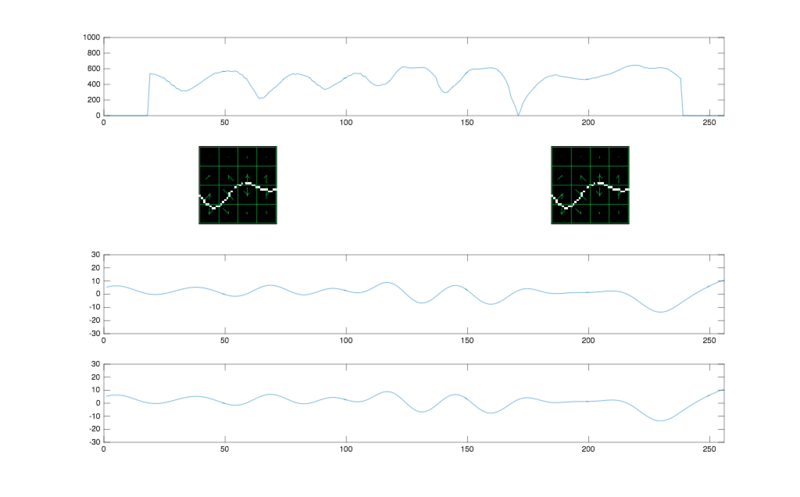
\includegraphics[scale=0.6]{images/dialdescriptores1.png}}
%\caption[Waveform identification Scheme]{Upper panel shows the euclidean distance between the descriptor 1 obtained from the left patch, and descriptor 2 obtained from the right patch.  Lower panels show the signal 1, which is used to generate the first descriptor and signal 2 which is used to generate the patch from the right.  The signals are exactly the same, hence the distance between descriptors is zero at exactly the keypoint position corresponding $175$ sample point.}
%\label{fig:dialdescriptors1}
%\end{figure}


%\begin{figure}[h!]
%\centering
%\subfigure[]
%{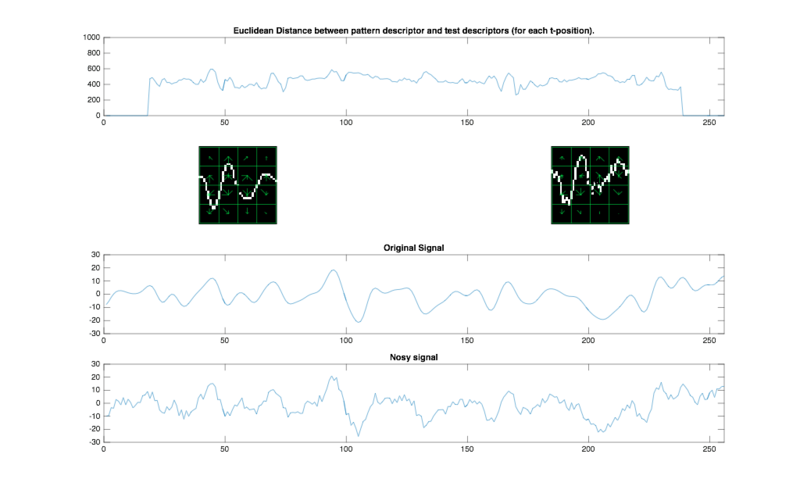
\includegraphics[scale=0.6]{images/dialdescriptores3.png}}
%\caption[Waveform identification under the presence of noisy signals]{In this case, the signal from the bottom panel has a superimposed additive artificial random noise of $5 \si{db}$.  Although the minimum value in the euclidean distance panel is still the correct localization of the waveform, there is a false positive which differs only $3\%$ of the real value. }
%\label{fig:dialdescriptors2}
%\end{figure}


%\begin{figure}[h!]
%\centering
%\subfigure[]
%{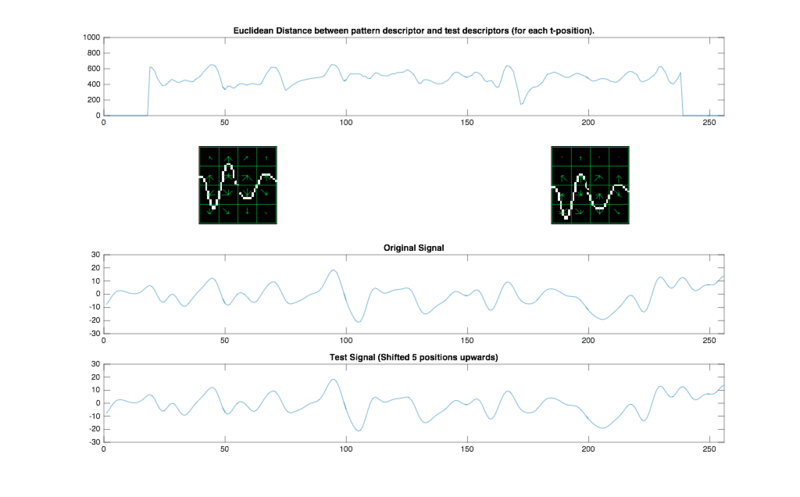
\includegraphics[scale=0.6]{images/dialdescriptores5.png}}
%\caption[Waveform identification under patch vertical translations]{If the keypoint is vertically translated 5 pixels downward or upward, the waveform can't no longer be identified correctly.}
%\label{fig:dialdescriptors5}
%\end{figure}


%\begin{figure}[h!]
%\centering
%\subfigure[]
%{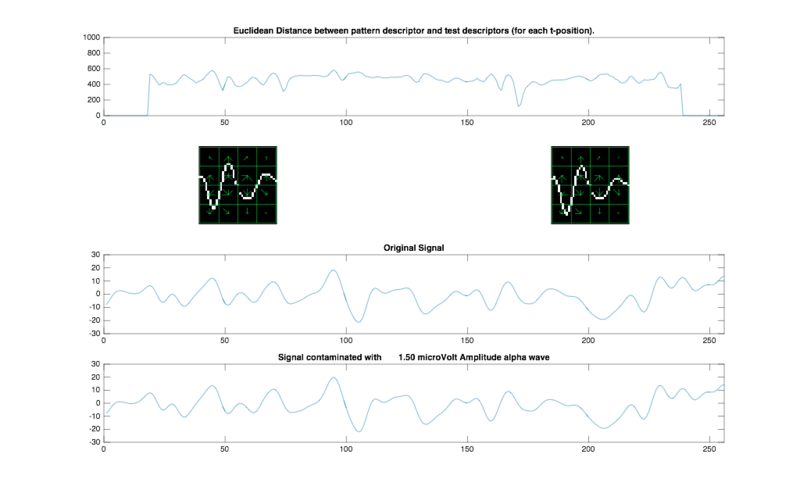
\includegraphics[scale=0.6]{images/dialdescriptores6.png}}
%\caption[Dial Descriptors 1]{With a subtle $1.5 \mu V$ noisy $10 Hz$ signal, there isn't changes.}
%\label{fig:dialdescriptors6}
%\end{figure}


%\begin{figure}[h!]
%\centering
%\subfigure[]
%{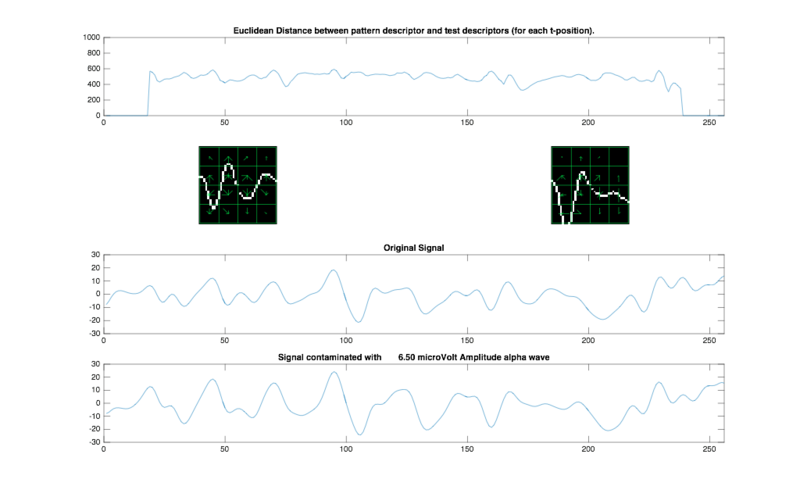
\includegraphics[scale=0.6]{images/dialdescriptores7.png}}
%\caption[Waveform identification under the presence of a noisy $\alpha$-wave.]{With a subtle $6.5 \mu V$ noisy $10 \si{Hz}$ signal, the waveform can no longer be localized effectively.}
%\label{fig:dialdescriptors7}
%\end{figure}

